\documentclass{standalone}
\usepackage{tikz}
\usetikzlibrary{patterns, positioning}


\begin{document}
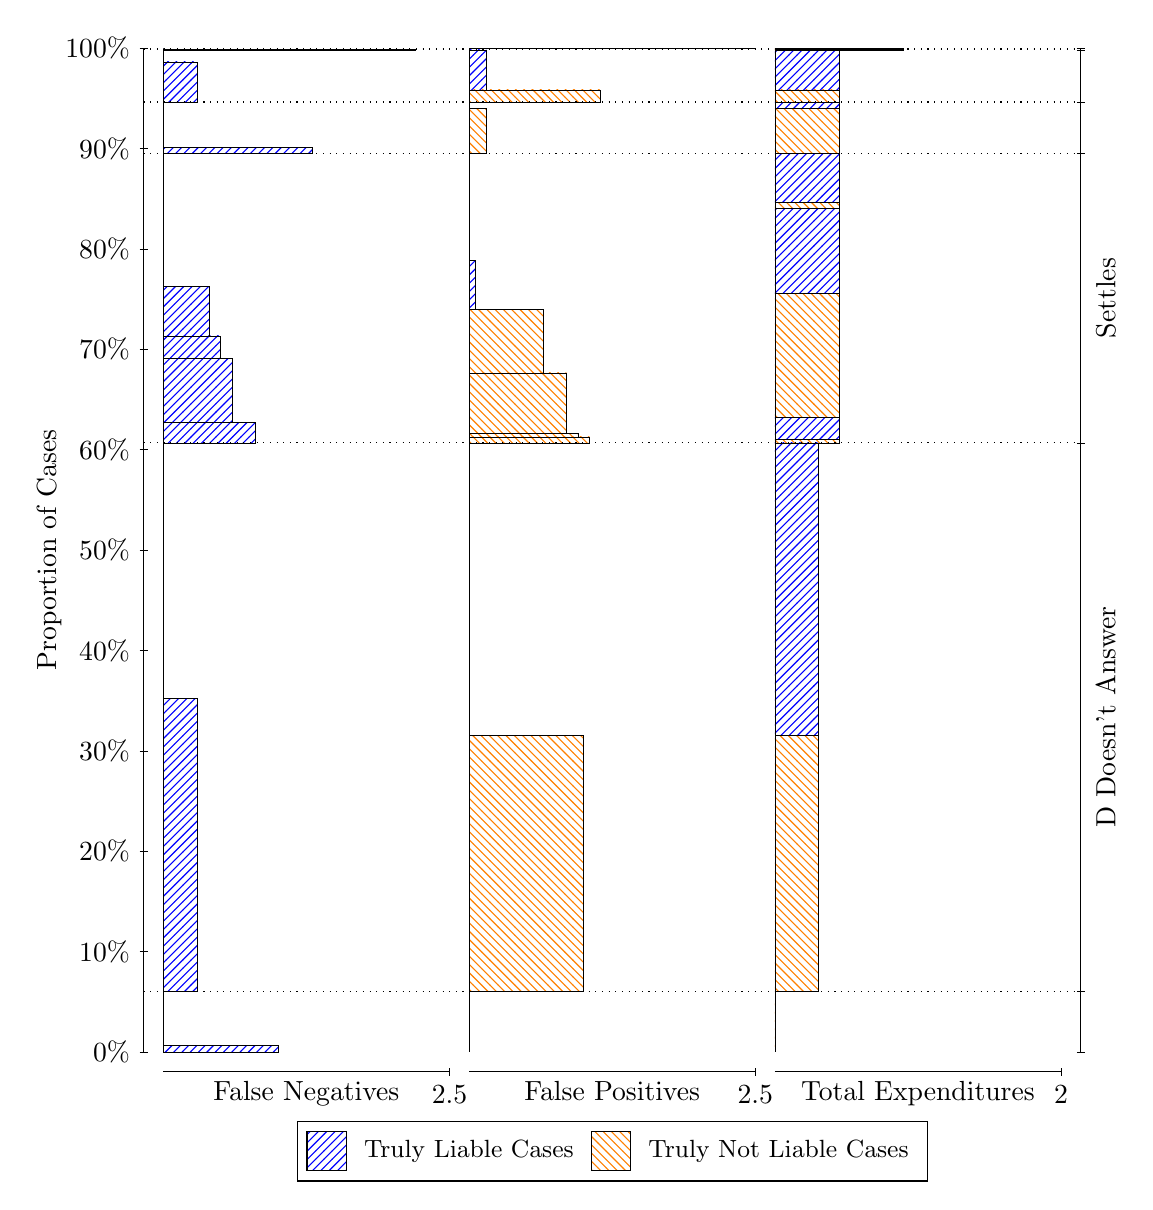
\begin{tikzpicture}
\draw[black, very thin] (1.5,1.75) -- (1.5,14.5);
\node[rotate=90, text=black, anchor=center] at (0.3, 8.125) {Proportion of Cases};
\draw[black, very thin] (1.45,1.75) -- (1.55,1.75);
\node[text=black, anchor=east] at (1.45, 1.75) {0\%};
\draw[black, very thin] (1.45,3.025) -- (1.55,3.025);
\node[text=black, anchor=east] at (1.45, 3.025) {10\%};
\draw[black, very thin] (1.45,4.3) -- (1.55,4.3);
\node[text=black, anchor=east] at (1.45, 4.3) {20\%};
\draw[black, very thin] (1.45,5.575) -- (1.55,5.575);
\node[text=black, anchor=east] at (1.45, 5.575) {30\%};
\draw[black, very thin] (1.45,6.85) -- (1.55,6.85);
\node[text=black, anchor=east] at (1.45, 6.85) {40\%};
\draw[black, very thin] (1.45,8.125) -- (1.55,8.125);
\node[text=black, anchor=east] at (1.45, 8.125) {50\%};
\draw[black, very thin] (1.45,9.4) -- (1.55,9.4);
\node[text=black, anchor=east] at (1.45, 9.4) {60\%};
\draw[black, very thin] (1.45,10.675) -- (1.55,10.675);
\node[text=black, anchor=east] at (1.45, 10.675) {70\%};
\draw[black, very thin] (1.45,11.95) -- (1.55,11.95);
\node[text=black, anchor=east] at (1.45, 11.95) {80\%};
\draw[black, very thin] (1.45,13.225) -- (1.55,13.225);
\node[text=black, anchor=east] at (1.45, 13.225) {90\%};
\draw[black, very thin] (1.45,14.5) -- (1.55,14.5);
\node[text=black, anchor=east] at (1.45, 14.5) {100\%};

\draw[black, very thin] (13.4,1.75) -- (13.4,14.5);
\draw[black, very thin] (13.35,1.75) -- (13.45,1.75);
\node[anchor=west] at (13.35, 1.75) {};
\draw[black, very thin] (13.35,2.5196) -- (13.45,2.5196);
\node[anchor=west] at (13.35, 2.5196) {};
\draw[black, very thin] (13.35,9.4863) -- (13.45,9.4863);
\node[anchor=west] at (13.35, 9.4863) {};
\draw[black, very thin] (13.35,13.164) -- (13.45,13.164);
\node[anchor=west] at (13.35, 13.164) {};
\draw[black, very thin] (13.35,13.814) -- (13.45,13.814);
\node[anchor=west] at (13.35, 13.814) {};
\draw[black, very thin] (13.35,14.477) -- (13.45,14.477);
\node[anchor=west] at (13.35, 14.477) {};
\draw[black, very thin] (13.35,14.492) -- (13.45,14.492);
\node[anchor=west] at (13.35, 14.492) {};
\draw[black, very thin] (13.35,14.5) -- (13.45,14.5);
\node[anchor=west] at (13.35, 14.5) {};

\draw[black, very thin, pattern color=blue, pattern=north east lines] (1.75,1.75) rectangle (3.2033,1.831);
\draw[black, very thin, pattern color=orange, pattern=north west lines] (1.75,1.831) rectangle (1.75,2.5196);
\draw[black, very thin, pattern color=blue, pattern=north east lines] (1.75,2.5196) rectangle (2.186,6.2371);
\draw[black, very thin, pattern color=orange, pattern=north west lines] (1.75,6.2371) rectangle (1.75,9.4863);
\draw[black, very thin, pattern color=blue, pattern=north east lines] (1.75,9.4863) rectangle (2.9127,9.7454);
\draw[black, very thin, pattern color=blue, pattern=north east lines] (1.75,9.7454) rectangle (2.622,10.562);
\draw[black, very thin, pattern color=blue, pattern=north east lines] (1.75,10.562) rectangle (2.4767,10.844);
\draw[black, very thin, pattern color=blue, pattern=north east lines] (1.75,10.844) rectangle (2.3313,11.468);
\draw[black, very thin, pattern color=orange, pattern=north west lines] (1.75,11.468) rectangle (1.75,13.164);
\draw[black, very thin, pattern color=blue, pattern=north east lines] (1.75,13.164) rectangle (3.6393,13.24);
\draw[black, very thin, pattern color=orange, pattern=north west lines] (1.75,13.24) rectangle (1.75,13.814);
\draw[black, very thin, pattern color=blue, pattern=north east lines] (1.75,13.814) rectangle (2.186,14.325);
\draw[black, very thin, pattern color=orange, pattern=north west lines] (1.75,14.325) rectangle (1.75,14.477);
\draw[black, very thin, pattern color=blue, pattern=north east lines] (1.75,14.477) rectangle (4.9473,14.481);
\draw[black, very thin, pattern color=orange, pattern=north west lines] (1.75,14.481) rectangle (1.75,14.492);
\draw[black, very thin, pattern color=orange, pattern=north west lines] (1.75,14.492) rectangle (1.75,14.495);
\draw[black, very thin, pattern color=blue, pattern=north east lines] (1.75,14.495) rectangle (1.75,14.5);
\draw[black, very thin, pattern color=orange, pattern=north west lines] (5.6333,1.75) rectangle (5.6333,2.4386);
\draw[black, very thin, pattern color=blue, pattern=north east lines] (5.6333,2.4386) rectangle (5.6333,2.5196);
\draw[black, very thin, pattern color=orange, pattern=north west lines] (5.6333,2.5196) rectangle (7.0867,5.7689);
\draw[black, very thin, pattern color=blue, pattern=north east lines] (5.6333,5.7689) rectangle (5.6333,9.4863);
\draw[black, very thin, pattern color=orange, pattern=north west lines] (5.6333,9.4863) rectangle (7.1593,9.5628);
\draw[black, very thin, pattern color=orange, pattern=north west lines] (5.6333,9.5628) rectangle (7.014,9.6063);
\draw[black, very thin, pattern color=orange, pattern=north west lines] (5.6333,9.6063) rectangle (6.8687,10.374);
\draw[black, very thin, pattern color=orange, pattern=north west lines] (5.6333,10.374) rectangle (6.578,11.182);
\draw[black, very thin, pattern color=blue, pattern=north east lines] (5.6333,11.182) rectangle (5.706,11.807);
\draw[black, very thin, pattern color=blue, pattern=north east lines] (5.6333,11.807) rectangle (5.6333,13.164);
\draw[black, very thin, pattern color=orange, pattern=north west lines] (5.6333,13.164) rectangle (5.8513,13.738);
\draw[black, very thin, pattern color=blue, pattern=north east lines] (5.6333,13.738) rectangle (5.6333,13.814);
\draw[black, very thin, pattern color=orange, pattern=north west lines] (5.6333,13.814) rectangle (7.3047,13.967);
\draw[black, very thin, pattern color=blue, pattern=north east lines] (5.6333,13.967) rectangle (5.8513,14.477);
\draw[black, very thin, pattern color=orange, pattern=north west lines] (5.6333,14.477) rectangle (5.6333,14.488);
\draw[black, very thin, pattern color=blue, pattern=north east lines] (5.6333,14.488) rectangle (5.6333,14.492);
\draw[black, very thin, pattern color=orange, pattern=north west lines] (5.6333,14.492) rectangle (9.2667,14.495);
\draw[black, very thin, pattern color=blue, pattern=north east lines] (5.6333,14.495) rectangle (7.8133,14.5);
\draw[black, very thin, pattern color=orange, pattern=north west lines] (9.5167,1.75) rectangle (9.5167,2.4386);
\draw[black, very thin, pattern color=blue, pattern=north east lines] (9.5167,2.4386) rectangle (9.5167,2.5196);
\draw[black, very thin, pattern color=orange, pattern=north west lines] (9.5167,2.5196) rectangle (10.062,5.7689);
\draw[black, very thin, pattern color=blue, pattern=north east lines] (9.5167,5.7689) rectangle (10.062,9.4863);
\draw[black, very thin, pattern color=orange, pattern=north west lines] (9.5167,9.4863) rectangle (10.334,9.5298);
\draw[black, very thin, pattern color=blue, pattern=north east lines] (9.5167,9.5298) rectangle (10.334,9.8114);
\draw[black, very thin, pattern color=orange, pattern=north west lines] (9.5167,9.8114) rectangle (10.334,11.387);
\draw[black, very thin, pattern color=blue, pattern=north east lines] (9.5167,11.387) rectangle (10.334,12.463);
\draw[black, very thin, pattern color=orange, pattern=north west lines] (9.5167,12.463) rectangle (10.334,12.54);
\draw[black, very thin, pattern color=blue, pattern=north east lines] (9.5167,12.54) rectangle (10.334,13.164);
\draw[black, very thin, pattern color=orange, pattern=north west lines] (9.5167,13.164) rectangle (10.334,13.738);
\draw[black, very thin, pattern color=blue, pattern=north east lines] (9.5167,13.738) rectangle (10.334,13.814);
\draw[black, very thin, pattern color=orange, pattern=north west lines] (9.5167,13.814) rectangle (10.334,13.967);
\draw[black, very thin, pattern color=blue, pattern=north east lines] (9.5167,13.967) rectangle (10.334,14.477);
\draw[black, very thin, pattern color=orange, pattern=north west lines] (9.5167,14.477) rectangle (11.152,14.488);
\draw[black, very thin, pattern color=blue, pattern=north east lines] (9.5167,14.488) rectangle (11.152,14.492);
\draw[black, very thin, pattern color=orange, pattern=north west lines] (9.5167,14.492) rectangle (11.152,14.495);
\draw[black, very thin, pattern color=blue, pattern=north east lines] (9.5167,14.495) rectangle (11.152,14.5);
\draw[black, dotted] (1.5,2.5196) -- (13.4,2.5196);
\draw[black, dotted] (1.5,9.4863) -- (13.4,9.4863);
\draw[black, dotted] (1.5,13.164) -- (13.4,13.164);
\draw[black, dotted] (1.5,13.814) -- (13.4,13.814);
\draw[black, dotted] (1.5,14.477) -- (13.4,14.477);
\draw[black, dotted] (1.5,14.492) -- (13.4,14.492);
\draw[black, very thin] (1.75,1.5) -- (5.3833,1.5);
\node[text=black, anchor=north] at (3.5667, 1.5) {False Negatives};
\draw[black, very thin] (5.3833,1.45) -- (5.3833,1.55);
\node[text=black, anchor=north] at (5.3833, 1.45) {2.5};

\draw[black, very thin] (5.6333,1.5) -- (9.2667,1.5);
\node[text=black, anchor=north] at (7.45, 1.5) {False Positives};
\draw[black, very thin] (9.2667,1.45) -- (9.2667,1.55);
\node[text=black, anchor=north] at (9.2667, 1.45) {2.5};

\draw[black, very thin] (9.5167,1.5) -- (13.15,1.5);
\node[text=black, anchor=north] at (11.333, 1.5) {Total Expenditures};
\draw[black, very thin] (13.15,1.45) -- (13.15,1.55);
\node[text=black, anchor=north] at (13.15, 1.45) {2};


\node[text=black, centered, rotate=90] at (13.72, 6.003) {D Doesn't Answer};
\node[text=black, centered, rotate=90] at (13.72, 11.325) {Settles};





\draw (7.449999999999999,1.5) node[draw=none] (baseCoordinate) {};
\begin{scope}[align=center]
        \matrix[scale=0.5, draw=black, below=0.5cm of baseCoordinate, nodes={draw}, column sep=0.1cm]{
            \node[rectangle, draw, minimum width=0.5cm, minimum height=0.5cm, pattern color=blue, pattern=north east lines] {}; &
            \node[draw=none, font=\small, text=black] (B) {Truly Liable Cases}; &
            \node[rectangle, draw, minimum width=0.5cm, minimum height=0.5cm, pattern color=orange, pattern=north west lines] {}; &
            \node[draw=none, font=\small, text=black] (B) {Truly Not Liable Cases}; \\
            };
\end{scope}

\end{tikzpicture}
\end{document}